
\subsection{N6 -- Phân tích gói tin bằng Wireshark}

\subsubsection{Mục tiêu}

Nhiệm vụ N6 nhằm phân tích hoạt động trao đổi thông tin
định tuyến của hai giao thức BGP và RIPv2 thông qua
các gói tin được bắt trực tiếp bằng Wireshark trong
môi trường mô phỏng GNS3.

Cụ thể, nhóm thực hiện:
\begin{itemize}
    \item Bắt và phân tích các bản tin BGP OPEN, UPDATE
    và KEEPALIVE trên liên kết L4 giữa A2 và B1.
    
    \item Phân tích các thuộc tính AS\_PATH, NEXT\_HOP
    và NLRI trong bản tin BGP UPDATE.
    
    \item Bắt các bản tin RIPv2 trên liên kết L1 giữa
    A1 và A2, đồng thời giải thích địa chỉ IP đích
    được sử dụng trong quá trình trao đổi thông tin
    định tuyến.
\end{itemize}

\subsubsection{Phương pháp thực hiện}

Nhóm sử dụng chức năng \textit{Start Capture} của GNS3
để bắt gói tin trên hai liên kết L4 và L1,
sau đó phân tích bằng phần mềm Wireshark.

\begin{table}[H]
    \centering
    \caption{Các liên kết được sử dụng trong thử nghiệm N6}
    \label{tab:n6-links}
    \renewcommand{\arraystretch}{1.3}
    \begin{tabular}{|c|l|l|l|}
        \hline
        \textbf{Link} &
        \textbf{Kết nối} &
        \textbf{Giao thức} &
        \textbf{Bộ lọc Wireshark} \\
        \hline
        L4 & A2 -- B1 & eBGP & \texttt{bgp} \\
        \hline
        L1 & A1 -- A2 & RIPv2 & \texttt{rip} \\
        \hline
    \end{tabular}
\end{table}

\paragraph{a) Bắt gói BGP trên L4}

Liên kết L4 kết nối router A2 thuộc AS 64626
với router B1 thuộc AS 64726.

Địa chỉ IP hai đầu liên kết:
\begin{itemize}
    \item A2 (Fa1/0): \texttt{10.71.26.13/30}.
    \item B1 (Fa0/0): \texttt{10.71.26.14/30}.
\end{itemize}

Sau khi kích hoạt Wireshark trên L4, nhóm sử dụng
bộ lọc \texttt{bgp} để quan sát các bản tin trao đổi.

Để thu thập bản tin OPEN và UPDATE trong quá trình
thiết lập phiên BGP, nhóm thực hiện thiết lập lại
phiên eBGP giữa A2 và B1 bằng lệnh:

\begin{verbatim}
clear ip bgp 10.71.26.13
\end{verbatim}

Lệnh được thực hiện trên router B1 sau khi
Wireshark đã bắt đầu ghi gói tin.

\paragraph{b) Bắt gói RIPv2 trên L1}

Liên kết L1 kết nối hai router A1 và A2
trong AS A, sử dụng giao thức RIPv2.

Địa chỉ IP hai đầu liên kết:
\begin{itemize}
    \item A1 (Fa0/0): \texttt{10.71.26.1/30}.
    \item A2 (Fa0/0): \texttt{10.71.26.2/30}.
\end{itemize}

Nhóm kích hoạt chức năng bắt gói trên L1 và
sử dụng bộ lọc \texttt{rip} để quan sát các
bản tin cập nhật định tuyến được gửi định kỳ.

\subsubsection{Kết quả phân tích}

\paragraph{a) Phân tích bản tin BGP OPEN}

Bản tin OPEN được sử dụng trong giai đoạn thiết lập
phiên BGP, cho phép hai router trao đổi các thông số
cần thiết trước khi hình thành quan hệ BGP Neighbor.

Kết quả Wireshark tại Frame 49 ghi nhận bản tin
OPEN được gửi từ A2 đến B1 với các thông tin sau:

\begin{table}[H]
    \centering
    \caption{Thông tin bản tin BGP OPEN trên L4}
    \label{tab:n6-bgp-open}
    \renewcommand{\arraystretch}{1.3}
    \begin{tabular}{|l|l|}
        \hline
        \textbf{Trường} & \textbf{Giá trị} \\
        \hline
        Source IP & 10.71.26.13 \\
        \hline
        Destination IP & 10.71.26.14 \\
        \hline
        BGP Version & 4 \\
        \hline
        Message Type & OPEN (1) \\
        \hline
        My Autonomous System & 64626 \\
        \hline
        Hold Time & 180 giây \\
        \hline
        BGP Identifier & 10.171.26.2 \\
        \hline
    \end{tabular}
\end{table}

Trong đó, trường \textit{My Autonomous System}
cho biết router A2 thuộc AS 64626,
còn \textit{BGP Identifier} là giá trị định danh
của A2 trong giao thức BGP.

Giá trị Hold Time bằng 180 giây thể hiện thời gian
giữ phiên được A2 đề xuất trong bản tin OPEN.
Phiên BGP sử dụng giá trị Hold Time đã thương lượng
giữa hai router.

\begin{figure}[H]
    \centering
    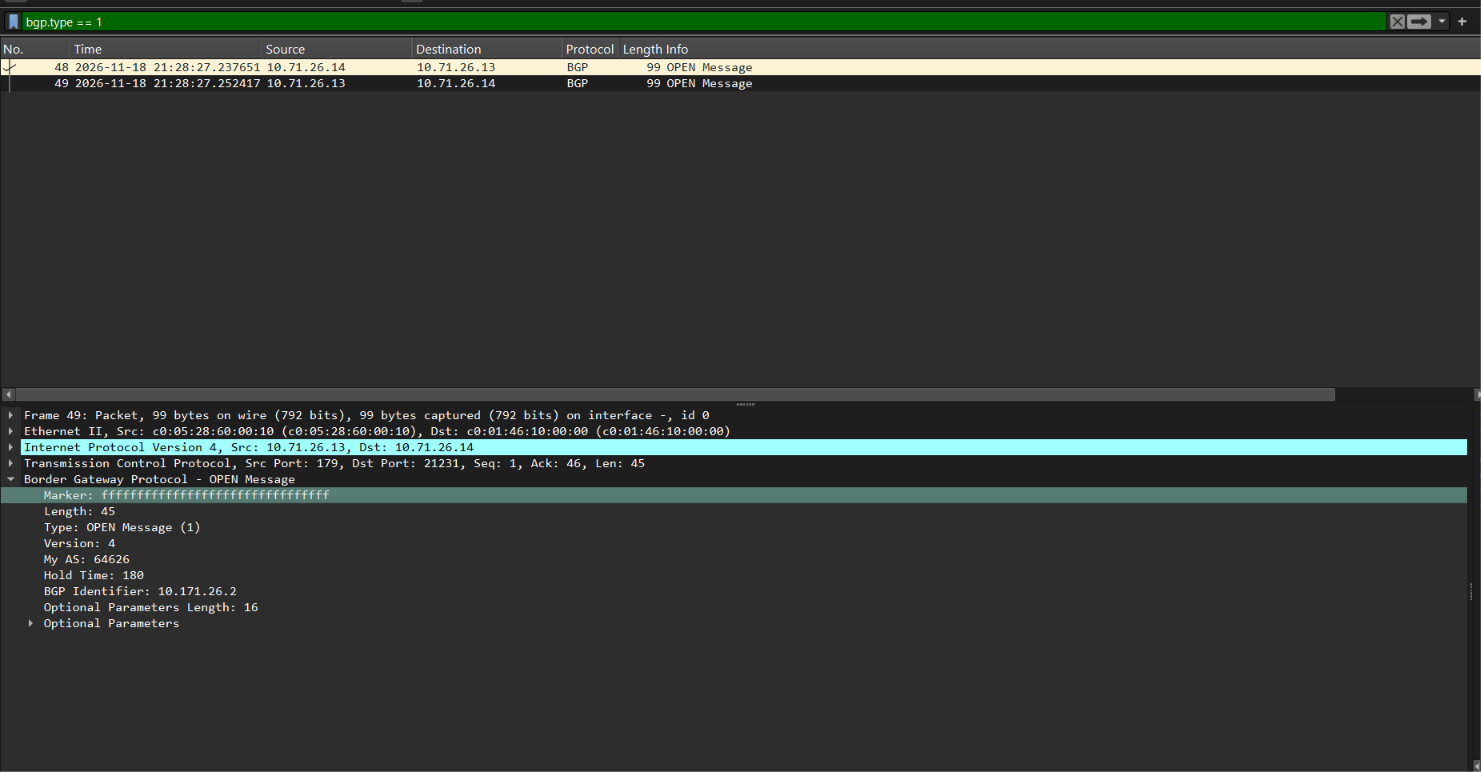
\includegraphics[width=0.95\textwidth]
    {images/advanced/N6/bgp_open.png}
    \caption{Phân tích bản tin BGP OPEN từ A2 đến B1
    trên liên kết L4}
    \label{fig:n6-bgp-open}
\end{figure}

\paragraph{b) Phân tích bản tin BGP UPDATE}

Bản tin UPDATE được sử dụng để quảng bá hoặc
thu hồi thông tin định tuyến BGP.

Tại Frame 53, Wireshark ghi nhận một bản tin
UPDATE được gửi từ A2 đến B1 với các thuộc tính:

\begin{table}[H]
    \centering
    \caption{Các thuộc tính trong bản tin BGP UPDATE}
    \label{tab:n6-bgp-update}
    \renewcommand{\arraystretch}{1.3}
    \begin{tabular}{|l|l|}
        \hline
        \textbf{Trường} & \textbf{Giá trị} \\
        \hline
        Source IP & 10.71.26.13 \\
        \hline
        Destination IP & 10.71.26.14 \\
        \hline
        Message Type & UPDATE (2) \\
        \hline
        ORIGIN & IGP \\
        \hline
        AS\_PATH & 64626 \\
        \hline
        NEXT\_HOP & 10.71.26.13 \\
        \hline
        MULTI\_EXIT\_DISC & 1 \\
        \hline
        NLRI & 10.171.126.0/26 \\
        \hline
    \end{tabular}
\end{table}

\textbf{Phân tích AS\_PATH:}

Thuộc tính AS\_PATH có giá trị \texttt{64626},
cho biết tuyến đang được quảng bá từ AS A
sang AS B.

AS\_PATH lưu thông tin các AS mà route đã đi qua,
đồng thời hỗ trợ BGP phát hiện vòng lặp định tuyến
giữa các Autonomous System.

\textbf{Phân tích NEXT\_HOP:}

Thuộc tính NEXT\_HOP có giá trị
\texttt{10.71.26.13}, tương ứng địa chỉ interface
Fa1/0 của A2 trên liên kết L4.

Điều này cho biết B1 có thể sử dụng A2 làm
next hop để chuyển tiếp lưu lượng đến mạng
được quảng bá.

\textbf{Phân tích NLRI:}

Trường NLRI chứa prefix
\texttt{10.171.126.0/26}, tương ứng với mạng LAN-A.

Như vậy, bản tin UPDATE cho thấy A2 đang quảng bá
mạng LAN-A đến B1 thông qua phiên eBGP giữa
AS 64626 và AS 64726.

\begin{figure}[H]
    \centering
    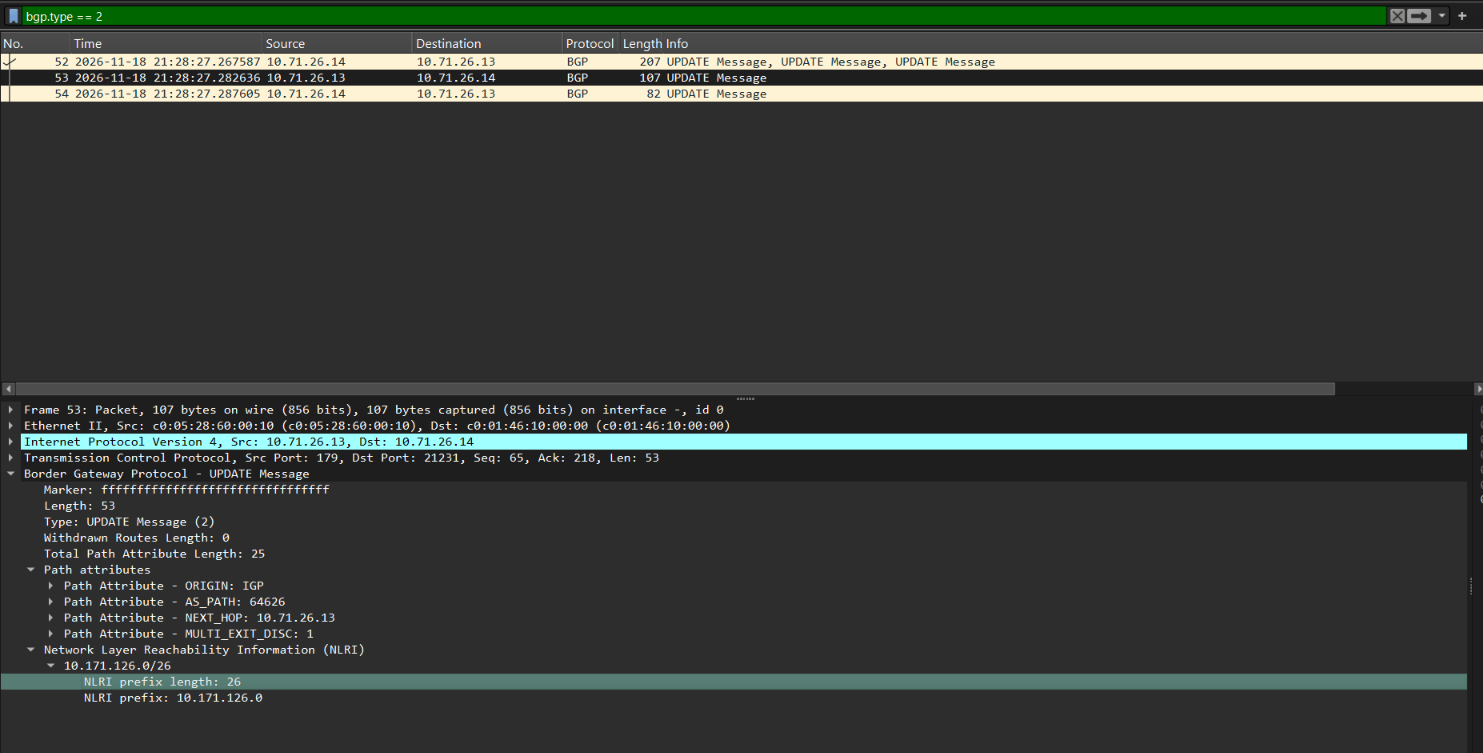
\includegraphics[width=0.95\textwidth]
    {images/advanced/N6/bgp_update.png}
    \caption{Phân tích bản tin BGP UPDATE với
    các thuộc tính AS\_PATH, NEXT\_HOP và NLRI}
    \label{fig:n6-bgp-update}
\end{figure}

Ngoài bản tin quảng bá route, Wireshark còn ghi nhận
một bản tin UPDATE tại Frame 54 dùng để thu hồi
prefix \texttt{10.171.126.0/26}.

Bản tin này chứa trường Withdrawn Routes
và không có Path Attributes, minh họa khả năng
thu hồi thông tin định tuyến của giao thức BGP.

\paragraph{c) Phân tích bản tin BGP KEEPALIVE}

Bản tin KEEPALIVE được sử dụng để duy trì
quan hệ BGP Neighbor khi phiên BGP đang hoạt động.

Tại Frame 110, Wireshark ghi nhận một bản tin
KEEPALIVE từ A2 đến B1.

\begin{table}[H]
    \centering
    \caption{Thông tin bản tin BGP KEEPALIVE}
    \label{tab:n6-bgp-keepalive}
    \renewcommand{\arraystretch}{1.3}
    \begin{tabular}{|l|l|}
        \hline
        \textbf{Trường} & \textbf{Giá trị} \\
        \hline
        Source IP & 10.71.26.13 \\
        \hline
        Destination IP & 10.71.26.14 \\
        \hline
        Message Type & KEEPALIVE (4) \\
        \hline
        BGP Message Length & 19 bytes \\
        \hline
    \end{tabular}
\end{table}

Bản tin KEEPALIVE có độ dài 19 bytes,
chỉ bao gồm phần header BGP và không mang
thông tin prefix định tuyến.

Việc các router trao đổi KEEPALIVE cho thấy
chúng đang duy trì liên lạc trong phiên BGP.

\begin{figure}[H]
    \centering
    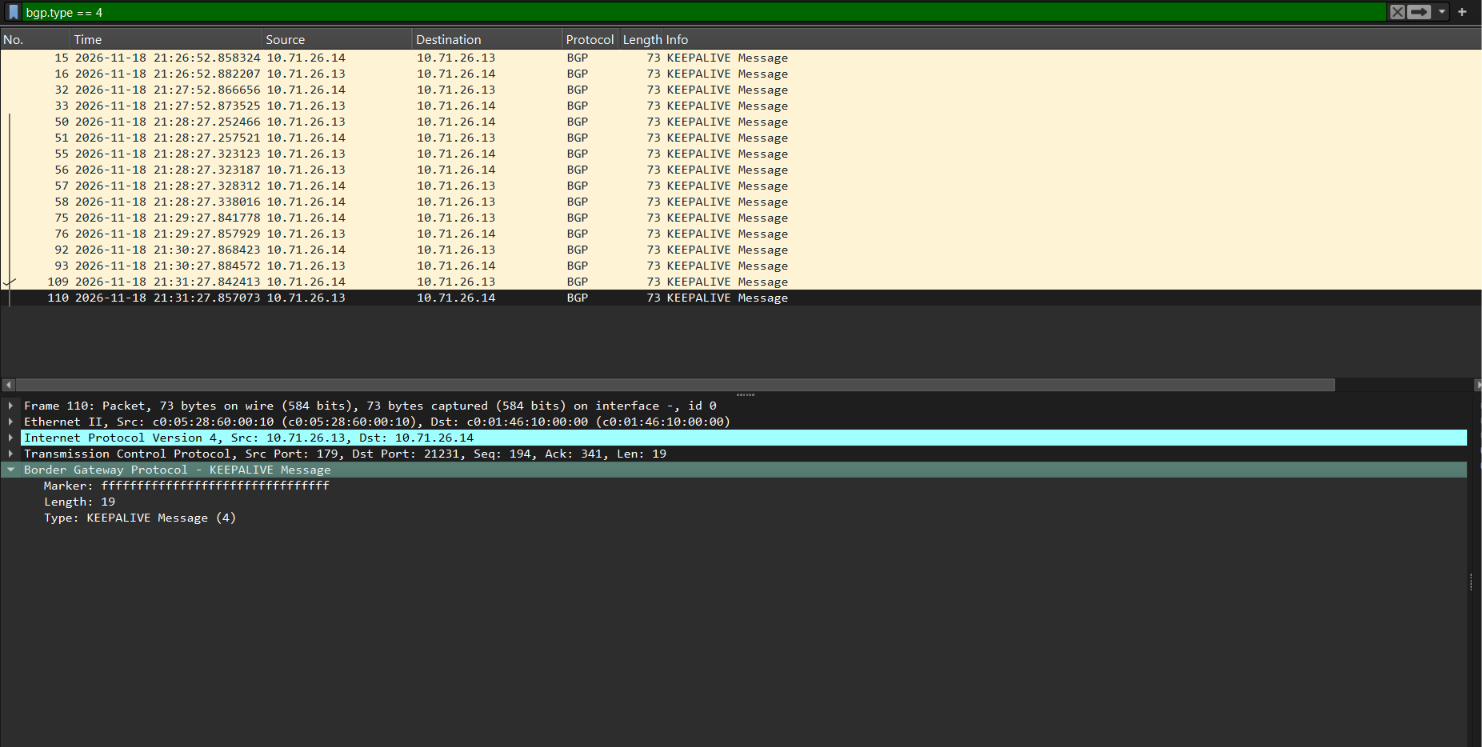
\includegraphics[width=0.95\textwidth]
    {images/advanced/N6/bgp_keepalive.png}
    \caption{Bản tin BGP KEEPALIVE giữa A2 và B1
    trên liên kết L4}
    \label{fig:n6-bgp-keepalive}
\end{figure}

\paragraph{d) Phân tích bản tin RIPv2 trên L1}

Kết quả Wireshark tại Frame 34 cho thấy router A2
gửi bản tin RIPv2 Response đến địa chỉ multicast
\texttt{224.0.0.9}.

Các thông tin chính được ghi nhận:

\begin{table}[H]
    \centering
    \caption{Thông tin bản tin RIPv2 Response trên L1}
    \label{tab:n6-rip}
    \renewcommand{\arraystretch}{1.3}
    \begin{tabular}{|l|l|}
        \hline
        \textbf{Trường} & \textbf{Giá trị} \\
        \hline
        Source IP & 10.71.26.2 \\
        \hline
        Destination IP & 224.0.0.9 \\
        \hline
        Transport Protocol & UDP \\
        \hline
        Source Port & 520 \\
        \hline
        Destination Port & 520 \\
        \hline
        Command & Response (2) \\
        \hline
        Version & RIPv2 (2) \\
        \hline
        \end{tabular}
\end{table}

\textbf{Phân tích địa chỉ đích:}

Địa chỉ \texttt{224.0.0.9} là địa chỉ multicast
được sử dụng bởi RIPv2 để gửi các bản tin cập nhật
định tuyến đến những router RIPv2 trên cùng liên kết.

Khác với RIPv1 sử dụng broadcast,
RIPv2 mặc định sử dụng multicast nhằm gửi thông tin
đến nhóm router tham gia giao thức.

Trong bản ghi Wireshark, nhóm quan sát được
các bản tin Response có địa chỉ nguồn
\texttt{10.71.26.1} và \texttt{10.71.26.2},
cho thấy A1 và A2 đều gửi thông tin RIP trên L1.

\textbf{Phân tích thông tin định tuyến:}

Bản tin RIPv2 chứa các route entry,
trong đó một entry được ghi nhận với thông tin:

\begin{table}[H]
    \centering
    \caption{Phân tích route entry trong bản tin RIPv2}
    \label{tab:n6-rip-entry}
    \renewcommand{\arraystretch}{1.3}
    \begin{tabular}{|l|l|}
        \hline
        \textbf{Trường} & \textbf{Giá trị} \\
        \hline
        Address Family & IP (2) \\
        \hline
        Route Tag & 0 \\
        \hline
        IP Address & 10.71.26.8 \\
        \hline
        Subnet Mask & 255.255.255.252 \\
        \hline
        Next Hop & 0.0.0.0 \\
        \hline
        Metric & 1 \\
        \hline
    \end{tabular}
\end{table}

Prefix \texttt{10.71.26.8/30} tương ứng với
mạng L3 giữa A2 và A3.

Giá trị Metric bằng 1 cho biết đây là tuyến
được A2 quảng bá với chi phí RIP là 1 hop.

Trường Next Hop bằng \texttt{0.0.0.0} cho biết
router nhận bản tin sử dụng router gửi cập nhật
làm next hop cho tuyến này.
Theo cơ chế của RIPv2, khi nhận được giá trị này,
router A1 sẽ sử dụng địa chỉ IP nguồn của bản tin
(\texttt{10.71.26.2}, thuộc A2) làm next hop
đối với tuyến được học.

Việc bản tin chứa đầy đủ địa chỉ mạng,
subnet mask, next hop và metric cho thấy RIPv2
hỗ trợ quảng bá thông tin định tuyến
theo cơ chế classless.

\begin{figure}[H]
    \centering
    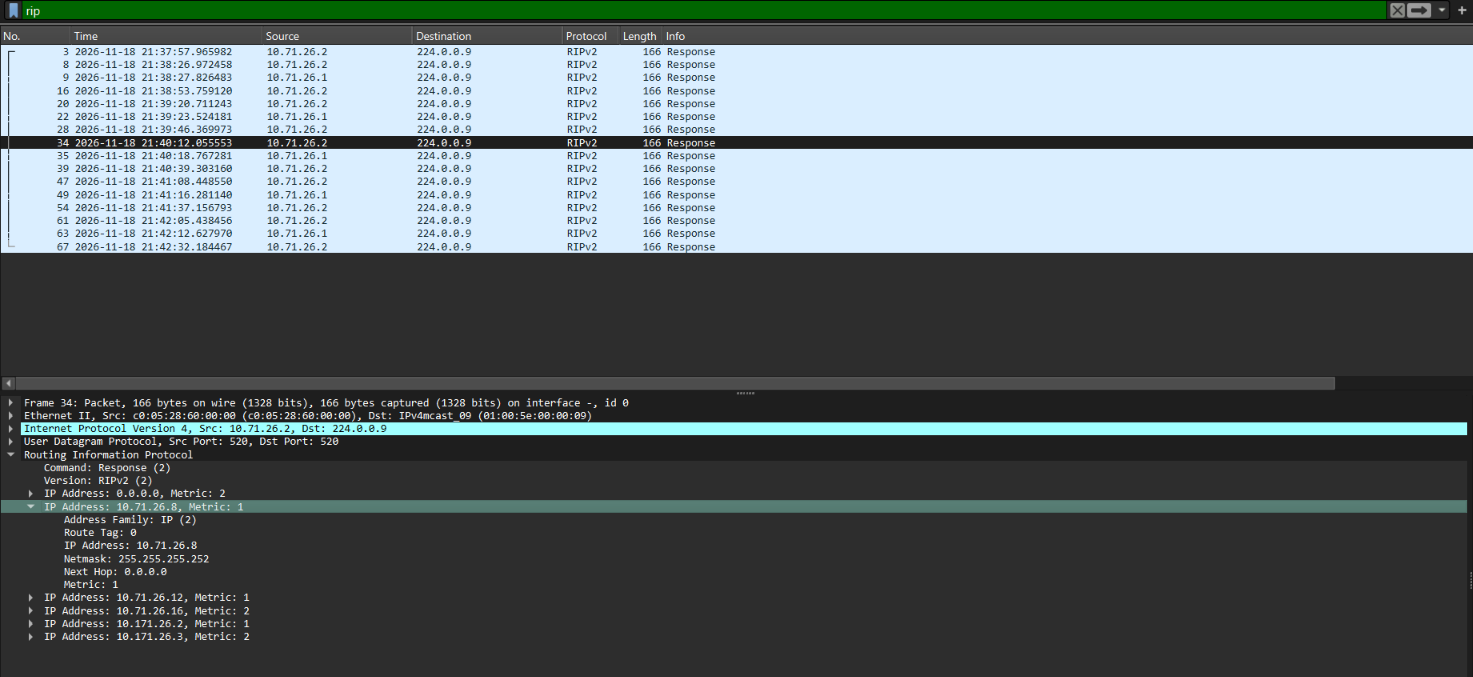
\includegraphics[width=0.95\textwidth]
    {images/advanced/N6/ripv2.png}
    \caption{Phân tích bản tin RIPv2 Response và
    route entry trên liên kết L1}
    \label{fig:n6-ripv2}
\end{figure}


